% CVPR 2026 Paper Template; see https://github.com/cvpr-org/author-kit

\documentclass[10pt,twocolumn,letterpaper]{article}

%%%%%%%%% PAPER TYPE  - PLEASE UPDATE FOR FINAL VERSION
\usepackage{cvpr}              % To produce the CAMERA-READY version
% \usepackage[review]{cvpr}      % To produce the REVIEW version
% \usepackage[pagenumbers]{cvpr} % To force page numbers, e.g. for an arXiv version

% Import additional packages in the preamble file, before hyperref
\input{preamble}

\usepackage{pifont}
\newcommand{\cmark}{\ding{51}} % checkmark
\newcommand{\xmark}{\ding{55}} % x-mark

% It is strongly recommended to use hyperref, especially for the review version.
% hyperref with option pagebackref eases the reviewers' job.
% Please disable hyperref *only* if you encounter grave issues,
% e.g. with the file validation for the camera-ready version.
%
% If you comment hyperref and then uncomment it, you should delete *.aux before re-running LaTeX.
% (Or just hit 'q' on the first LaTeX run, let it finish, and you should be clear).
\definecolor{cvprblue}{rgb}{0.21,0.49,0.74}
\usepackage[pagebackref,breaklinks,colorlinks,allcolors=cvprblue]{hyperref}
\usepackage{amsthm}
% Numbering propositions, theorems, lemmas, corollaries within sections
\newtheorem{theorem}{Theorem}[section]
\newtheorem{proposition}[theorem]{Proposition}
\newtheorem{lemma}[theorem]{Lemma}
\newtheorem{corollary}[theorem]{Corollary}

% Definitions, remarks, examples in a different style (upright)
\theoremstyle{definition}
\newtheorem{definition}[theorem]{Definition}
\newtheorem{example}[theorem]{Example}

\theoremstyle{remark}
\newtheorem{remark}[theorem]{Remark}

%%%%%%%%% PAPER ID  - PLEASE UPDATE
\def\paperID{23419} % *** Enter the Paper ID here
\def\confName{CVPR}
\def\confYear{2026}

%%%%%%%%% TITLE - PLEASE UPDATE
\title{The Selective Disk Bispectrum and Its Inversion, with Application to Multi-Reference Alignment}

%%%%%%%%% AUTHORS - PLEASE UPDATE
\author{Adele Myers Lantow\\
UC Santa Barbara\\
{\tt\small adele@ucsb.edu}
% For a paper whose authors are all at the same institution,
% omit the following lines up until the closing ``}''.
% Additional authors and addresses can be added with ``\and'',
% just like the second author.
% To save space, use either the email address or home page, not both
\and
Nina Miolane\\
UC Santa Barbara\\
{\tt\small ninamiolane@ucsb.edu}
}

\begin{document}
\maketitle
\begin{abstract}
In many computer vision and shape analysis tasks, practitioners are interested in learning from the \textit{shape} of the object in an image, while disregarding the object's orientation. To this end, it is valuable to define a \textit{rotation-invariant} representation of images, retaining all information about that image, but disregarding the way an object is rotated in the frame. To be practical for learning tasks, this representation must be \textit{computationally efficient} for large datasets and \textit{invertible}, so the representation can be visualized in image space. To this end, we present the selective disk bispectrum: a fast, rotation-invariant representation for image shape analysis. While the translational bispectrum has long been used as a translational invariant representation for 1D and 2D signals, its extension to 2D (disk) rotational invariance on images has been hindered by the absence of an invertible formulation and its cubic complexity. In this work, we derive an explicit inverse for the disk bispectrum, which allows us to define a ``selective" disk bispectrum, which only uses the minimal number of coefficients needed for faithful shape recovery. We show that this representation enables multi-reference alignment for rotated images—a task previously intractable for disk bispectrum methods. These results establish the disk bispectrum as a practical and theoretically grounded tool for learning on rotation-invariant shape data.
\end{abstract}

\section{Introduction}
The translation-invariant bispectrum is a higher-order spectral representation that originated in the mid-20th century for signal processing \citep{tukey1953spectral, brillinger1991some, nikias1993signal}. Unlike the power spectrum, which captures second-order (pairwise) correlations between Fourier coefficients, the bispectrum encodes third-order relationships, making it sensitive to asymmetries and nonlinear interactions in the signal. More importantly, unlike the power spectrum which drops the phase of the signal, the translation-invariant bispectrum conserves everything about the signal except for its global phase, making it a \textit{complete} translational invariant.

As a result, the translation-invariant bispectrum has found widespread applications across disciplines: oceanographers use it to analyze wave interactions~\citep{elgar1985observations}, seismologists to identify complex waveforms~\citep{geophysics_2004}, and biomedical engineers to study electroencephalograms~\citep{zhang2000bispectrum} as well as heart rate variability~\citep{martin2021bispectral}. It is similarly used in optical interferometry~\citep{Gordon_2012}, radar communications~\citep{liu2023modulation} and other applications as a way to identify patterns in 1D signals (see \cite{koukiou2024identifying} for a recent review). Such applications are only interested in translation invariance in 1D or 2D signals (images).

In contrast, other applications are interested in rotation invariance, and despite the widespread applicability and utilization of the 1D/2D translation-invariant bispectrum, the 2D rotation-invariant bispectrum has been under-developed. In many applications, key information lies in the \textit{shape} of a 2D image, and its orientation is a nuisance variable. Without an easily computable rotation invariant representation, practitioners must register each image before analysis.

To this end, \cite{zhao2014rotationally} proposed the disk bispectrum, which is invariant to 2D planar (disk) rotations. However, because they did not derive a bispectrum inversion, their analysis was restricted to classification problems in bispectrum space. For example, tasks like multi reference alignment (MRA) would be impossible. MRA estimates a ground truth signal by mapping shifted noisy versions of that signal into bispectrum space, averaging the signals in bispectrum space, and then inverting the average back to image space, which would be impossible without a bispectrum inversion. Additionally \cite{zhao2014rotationally}'s disk bispectrum was computationally expensive. Authors reported a cubic complexity of $\mathcal{O}(m^3 / N_{m})$ , where $m$ is the number of ``disk harmonic frequencies'', and $N_m$ the maximum frequency. Lastly, they resorted to principal component analysis (PCA) in bispectrum space to reduce its dimensionality. Authors do not prove completeness of the disk bispectrum or their PCA reduction, meaning it was unclear whether the bispectrum actually described all information about the original image up to a rotation.

In this work, we propose the first computationally tractable disk bispectrum, the \textit{selective disk bispectrum}, and its inversion, for use in image processing and shape analysis. We also provide a method for approximating the disk bispectrum, building on \cite{fast_dhcs_2023}.  Then, following \cite{bendory2018bispectrum}, we derive an MRA-specific disk bispectrum inversion, which corrects for noise propagation during disk bispectrum averaging, and demonstrate its efficacy on rotated noisy MNIST images.

\begin{figure*}[t]
  \centering
  \includegraphics[width=\textwidth]{figs/overview_figure.pdf}
  \caption{We propose the selective disk bispectrum, which reduces the time complexity of the disk bispectrum from $\mathcal{O}(m^3/N_m)$ to $\mathcal{O}(m)$, where $m$ is the number of disk harmonic frequencies, and $N_m$ the maximum frequency. We provide the first inversion of the disk bispectrum from its coefficients back to image space.}
  \label{fig:overview}
\end{figure*}


\textbf{Contributions}
\begin{enumerate}[leftmargin=*]
\item We introduce the \textit{selective disk bispectrum}, an efficient formulation that proves and exploits the redundancy of disk bispectral coefficients. This reduces the space complexity from $\mathcal{O}(m^3/N_m)$ to $\mathcal{O}(m)$ and the time complexity from $\mathcal{O}(L^3+m^3/N_m)$ to  $\mathcal{O}(L^3 + m)$, where $L \times L$ is the image size, $L^2$ is the number of total pixels, $m$ is the number of disk harmonic frequencies, and $N_m$ the maximum frequency. The selective disk bispectrum offers an \textit{efficient} rotation-invariant representation, making it scalable for large amounts of data.

\item We derive the first disk bispectrum inversion, mapping (selective) disk bispectrum coefficients back to image space. The value of this inversion is twofold. First, it enables practitioners to reconstruct an image from statistical results (such as computation of the mean) in disk bispectrum space, which is essential for interpretability. Second, the inversion proves that the selective disk bispectrum is a \textit{complete rotational invariant} for images on the disk, i.e., it preserves all information about an image up to a disk rotation. By association, it also provides the first completeness proof for the full disk bispectrum.

\item We provide a numerical approximation of the selective disk bispectrum, that further reduces its time complexity from $\mathcal{O}(L^3 + m)$ to $O(L^2\log L + m)$. We prove precise accuracy guarantees on this approximation.

\item We provide an open-source, unit-tested implementation of the selective disk bispectrum and its inversion in Python, along with its application to multi-reference alignment. We use this implementation to illustrate the forward and inverse selective disk bispectrum map (between images and coefficients), and compare against the full disk bispectrum map. We empirically demonstrate that the selective disk bispectrum can be used for multi-reference alignment on rotated images.

\end{enumerate}

In summary, the selective disk bispectrum offers a fast (scalable) and invertible (interpretable) tool for imaging applications involving rotation-invariant 2D shape analysis.

\section{Related Works}

\paragraph{Equivariant and Invariant Representations.} As geometric learning has gained popularity \cite{bronstein2021geometricdeeplearninggrids}, there has been increased interest in rotation-equivariant and rotation-invariant image representations. Put simply (and described later in more detail), if a representation is \textit{equivariant} to rotation, the representation changes in a specific way when the original image is rotated. If a representation is rotation \textit{invariant}, the representation does not change if the original image is rotated.

Table \ref{tab:rotation-summary} summarizes rotation equivariant and rotation invariant representations, showing that only our selective disk bispectrum is rotation invariant and invertible, making it the only method capable of multi-reference alignment on rotated images. As an aside, we note that every rotation-equivariant neural network (and every rotation-equivariant layer) can be made rotation-invariant by adding an invariant aggregation function, like the sum or the max, after it. However, because the sum or max cannot be inverted to reconstruct the input, this invariant shape descriptor is not invertible.


\begin{table}[t]
\centering
\footnotesize
\setlength{\tabcolsep}{4.5pt}
\renewcommand{\arraystretch}{1.15}
\begin{tabular}{lccccc}
\toprule
\textbf{Method} &
\textbf{Equiv.} &
\shortstack{\textbf{Local}\\\textbf{Inv.}} &
\shortstack{\textbf{Global}\\\textbf{Inv.}} &
\shortstack{\textbf{Mag.}\\\textbf{Inv.}} &
\shortstack{\textbf{Invertible}\\\textbf{Inv. Rep.}} \\
\midrule
\textbf{SDB(ours)} & \xmark & \cmark & \cmark & \cmark & \cmark \\
DH Tr. \cite{marshall2022fast} & \cmark & \xmark & \xmark & \xmark & \xmark \\
Log-Polar Tr. \cite{reddy1996fft} & \cmark & \xmark & \xmark & \cmark & \xmark \\
Fourier Mellin Tr. \cite{reddy1996fft} & \cmark & \xmark & \xmark & \cmark & \xmark \\
\shortstack{SIFT / SURF/ \\ORB / AKAZE\\ \cite{lowe2004sift,bay2006surf,rublee2011orb,alcantarilla2012kaze}}  & \xmark & \cmark & \xmark & \xmark & \xmark \\
Hu Moments \cite{hu1962visual} & \xmark & \cmark & \cmark & \xmark & \xmark \\
Zernike Moments \cite{teague1980zernike} & \xmark & \xmark & \xmark & \cmark & \xmark \\
TFNs \cite{thomas2018tfns} & \cmark & \xmark & \xmark & \cmark & \xmark \\
Spherical convs. \cite{cohen2018spherical,esteves2018spherical}& \cmark & \xmark & \xmark & \xmark & \xmark \\
Capsule Networks \cite{sabour2017dynamic} & \cmark & \xmark & \xmark & \xmark & \xmark \\
\bottomrule
\end{tabular}

\caption{Comparison of equivariance, invariance, and invertibility properties across image descriptors. Abbreviations: TFN Tensor Field Networks, Tr. Transform, Inv. Invariant, Equiv. Equivariant, SIFT Scale–Invariant Feature Transform, SURF Speeded–Up Robust Features, ORB Oriented FAST and Rotated BRIEF, AKAZE Accelerated KAZE.}
\label{tab:rotation-summary}
\end{table}


\paragraph{$G$-bispectra and their inversions.} \citet{kakarala_thesis} proposed the $G$-Bispectrum, defined for a signal whose domain is a group. The $G$-Bispectrum gained interest as it is the lowest-degree spectral invariant that is complete. The translation-invariant bispectrum, invariant to the cyclic group $G=C_n$, is a classic and widely used signal processing tool, and is an example of a $G$-bispectrum. \cite{giannakis1989} proposed the first inversion scheme of the translation-invariant bispectrum, reconstructing a 1D signal analytically from translation bispectrum coefficients. \cite{sundaramoorthy1990} developed another analytical inversion algorithm that is more robust to noise, and \cite{pinilla2023} revisited this inversion problem, providing a gradient-based inversion procedure. \cite{giannakis1989} also extended his 1D inversion scheme to invert the 2D translation-invariant bispectrum, invariant to the product of cyclic groups $C_n \times C_n$. The 2D translation-invariant bispectrum is another example of a $G$-Bispectrum.  \cite{ mataigne2024selective} generalized that proof for the product of any number of cyclic groups, \textit{i.e.}, to any $G$-bispectrum, for signals defined over a finite and commutative group $G$. A reflection-invariant bispectrum was also proposed by Edidin and Katz \cite{edidin2025}, who formulated a gradient descent optimization for its inversion. Methods to invert the $G$-bispectrum of signals defined on a (continuous) Lie group $G$ have been proposed in \cite{kakarala2012,kakarala1993}. Note, the disk bispectrum is not covered under any of the aforementioned proofs, as the signal is defined over a planar disk, which is not a group.

The $G$-bispectrum on homogeneous spaces, defined for a signal whose domain is homogeneous for a group $G$, was proposed by \cite{kakarala2012bispectrumsourcephasesensitiveinvariants}. A space that is homogeneous for a group is one where for any $x, y$ there is a group element $g \in G$ s.t. $g \circ x = y$. \cite{kakarala2012bispectrumsourcephasesensitiveinvariants} also proposed a method to invert the $G$-bispectrum of signals defined on spaces homogeneous for a group $G$, specifically for the sphere $S^2$, which is homogeneous for $SO(3)$. Existing rotation-invariant $G$-bispectra are defined for signals on the circle ($SO(2)$) or the sphere ($SO(3)$). Note, the disk bispectrum is not covered under any of these proofs, as the signal is defined over a planar disk, which is not homogeneous for the rotation group $SO(2)$.

\paragraph{Selective $G$-Bispectra.} Across existing $G$-bispectra, several authors have shown that bispectrum coefficients are generally redundant. It is usually possible to recover the signal with significantly fewer bispectrum coefficients than those provided in the full bispectrum, thus enabling a \textit{selective} version of that bispectrum. The work of \citep{giannakis1989signal, kakarala_thesis, sadler1992shift} showed that for \textit{some} finite, commutative groups, the $G$-Bispectrum can be computed with only $|G|$ space complexity, where $|G|$ is the number of elements in the group $G$. \citet{  mataigne2024selective} extended these results by showing this result for a wider range of finite groups, \textit{i.e.}, all discrete commutative groups, and some non-commutative ones such as the dihedral groups of any order, the octahedral and full octahedral group. \cite{ mataigne2024selective} further proposed inversion of selective bispectra for the following non-commutative groups: any dihedral group, the octahedral group, and the full octahedral group. \cite{  mataigne2024selective} estimates bispectra (for signals defined on a group) via a group convolution, and offers an algorithm that can be used to identify selective coefficients. In contrast, the disk bispectrum provides an analytic map from the image to the bispectrum coefficients and is defined for signals defined over the full disk, so that it can be applied to images. Additionally, our disk bispectrum inversion identifies the exact selective coefficients required for complete bispectrum inversion. In fact, this work is the first to introduce a selective bispectrum and inversion proof for a non-homogeneous bispectrum.

\paragraph{A Disk Bispectrum.} Most relevant to our work is the work by \citet{zhao2014rotationally}, who proposed the first disk bispectrum. As described in introduction, this full disk bispectrum is impracticable due to its cubic complexity and lack of inversion, which is why we propose the selective disk bispectrum and its inversion.

Related to our work, Kakarala \cite{kakarala2012} proposes inverting a non-complete bispectrum-like function on the disk by introducing an auxiliary function that supplies the missing information needed for reconstruction and using the inversion method of the cyclic group. In contrast, our disk bispectrum inversion is complete and requires no external information to reconstruct the original image from bispectral coefficients.

\paragraph{Multi-reference alignment} We will show the utility of our bispectrum and its inversion to perform multi-reference alignment (MRA). Traditional \textit{translational} MRA utilizes the translation bispectrum, but special methods are required to adjust for a bias induced by noise in bispectrum space. Various techniques have been proposed for this task, such as noise bias estimation and correction \cite{bendory2018bispectrum}, spectral initialization approaches to MRA optimization \cite{chen2018spectral}, and Gauss–Newton optimization schemes \cite{herring2019gauss}. These corrections, however, have been derived only for the \textit{1D translation bispectrum}. No such correction has been established for the \textit{disk bispectrum}. In this work, we not only propose the \textit{selective disk bispectrum}, its inversion, and its approximation, but we also derive the corresponding MRA noise correction term in a similar manner to \cite{bendory2018bispectrum}. Notably, MRA with the disk bispectrum would not be possible without our inversion method, since reconstructing the mean bispectrum back to image space requires a well-defined inverse.

\section{Background}
\paragraph{Disk Harmonics.}
The 1D translation bispectrum (which is invariant to group action on the circle $S^1$) is composed of Fourier coefficients, which are constructed using Fourier modes, which are eigenfunctions of the Laplacian on $S^1$. Thus, naturally, if we wish to compose a bispectrum invariant to disk rotations, we should do so with disk harmonic coefficients, which are constructed using disk harmonics, which are the eigenfunctions of the Laplacian on the unit disk $\mathbb{D} = \{ x \in \mathbb{R}^2 : \|x\| < 1 \}$. In polar coordinates \( (r, \theta) \in [0,1) \times [0, 2\pi) \), these disk harmonics are given by
\[
\psi_{nk}(r, \theta) = c_{nk} J_n(\lambda_{nk} r) e^{in\theta}
\]
where \( (n, k) \in \mathbb{Z} \times \mathbb{Z}_{>0} \), \( J_n \) is the $n$-th order Bessel function of the first kind, \( \lambda_{nk} \) is its \( k \)-th root of the $n$-th Bessel function, and \( c_{nk} \) is a normalization constant. Thus, radially, $\psi_{nk}(r, \theta)$ looks like a Bessel function whose value is \( \lambda_{nk} \) on the edge of the disk, and angularly, $\psi_{nk}(r, \theta)$ looks like a complex sinusoid.

\paragraph{Disk Harmonic (DH) Transform.} Let $f : \mathbb{D} \to \mathbb{R}$ be a real-valued square integrable function defined on the unit disk. Disk harmonics form an orthonormal basis for square-integrable functions (like Fourier modes), such that $f$ can be expanded as
$f(r, \theta) = \sum_{n \in \mathbb{Z}} \sum_{k \in \mathbb{Z}_{>0}} a_{nk} \, \psi_{nk}(r, \theta)$,
where $a_{nk} \in \mathbb{C}$ are \textit{disk harmonic (DH) coefficients}. The \textit{disk harmonic (DH) transform} computes these coefficients, expanding $f$ in the disk harmonic basis (akin to the Fourier transform expanding $f$ in the Fourier mode basis). A single coefficient, given by
\[
a_{nk} = \int_0^{2\pi} \int_0^1 f(r, \theta) \, \overline{\psi_{nk}(r, \theta)} \, r \, dr \, d\theta,
\]
encodes the amplitude and phase of $\psi_{nk}$, necessary to reconstruct the signal from the expansion equation above. Importantly, DH coefficients are \textit{equivariant} to rotation of $f$, meaning that a rotation in $f$ will correspond to a rotation in the DH coefficients of $f$.

\begin{proposition}[Equivariance]
More formally, denote $SO(2)$ the group of 2D rotations. Consider $f$ a square-integrable function on the unit disk with DH coefficients $\{a^f_{n, k}\}_{n\in \mathbb{Z}, k\in \mathbb{Z}_{>0}}$. For every $\phi \in SO(2)$, if $f' = f \circ R_\phi$, then for all $n, k \in \mathbb{Z} \times \mathbb{Z}_{>0}$, we have: $a^{f'}_{n, k} = e^{in\phi}\cdot a^{f}_{n, k}.$ Thus, the DH coefficients are equivariant to 2D rotations.
\end{proposition}

In the general case, a function $f$ is \textit{equivariant} to a transformation group $G$ if
\[
f(T_g x) = T_g' f(x), \quad \forall g \in G,
\]
where $T_g$ acts on the input and $T_g'$ is a corresponding action on the output. A function $f$ is \textit{invariant} to $G$ if
\[
f(T_g x) = f(x), \quad \forall g \in G.
\]
\paragraph{Signal Discretization on images.} While the disk harmonics are defined for functions $f : \mathbb{D} \to \mathbb{R}$, practical applications require discretization. We will work with discretized images, i.e., arrays of size $L \times L$ whose pixel values are interpreted as samples of $f$.
Let $p = L^2$ be the total number of pixels such that locations and values of image intensities are denoted as $x_1, \dots, x_p$ and $f_1, \dots, f_p$, respectively. For images of shape \( L \times L \) with spacing \( \Delta x = 2/L \), corresponding to the domain \( [-1,1] \times [-1,1] \), the sampling rate is \( (\Delta x)^{-1} = L/2 \), yielding a Nyquist frequency (i.e., bandlimit) of \( L/4 \). The \textit{Nyquist frequency} is the highest frequency that can be well represented when the signal is sampled at a given rate.

Recall that $\lambda_{nk}$ is the $k$-th root of the $n$-th order Bessel function, and that the disk harmonic $\psi_{nk}$ does not extend radially past $\lambda_{nk}$. Therefore, $\lambda_{nk}$ determines  the number of Bessel function oscillations over the disk and is therefore a quasi-frequency, which is subject to Nyquist criterion. According to the Nyquist criterion, we should only keep the DH coefficients for which $\frac{\lambda_{nk}}{2\pi} \leq \frac{L}{4}$, as higher-frequency components correspond to features beyond the image resolution~\citep{zhao2013fourier}.

\paragraph{Truncation of DH coefficients.} Following closely with \cite{fast_dhcs_2023}, for a given bandlimit $\lambda > 0$, typically $\lambda = \frac{\pi L}{2}$, we keep the DH coefficients for indices $(n,k)$ such that $\lambda_{nk} \leq \lambda$, and order them from lowest frequency to highest $\lambda_0 \leq \cdots \leq \lambda_{m-1}$. The index $j=0, ..., m-1$ represents this order. As such, we now index $\lambda_j$ or equivalently $\lambda_{n_j,k_j}$, where $n_j, k_j$ are the $n,k$ of the frequency at index $j$. Importantly, Bessel function roots do not repeat over order, so we can uniquely identify a disk harmonic via $\lambda_{n_j,k_j}$. As such, we also index $\psi$ by $j$, denoting $\psi_j = \psi_{n_j k_j}$.

Table~\ref{tab:indices} shows the indices $j=0, ..., m-1$ organized in a table labeled by $n, k$ for an image of size $8 \times 8$ and $\lambda = \frac{\pi L}{2}$. Further, for a given bandwidth $\lambda$ that determines a number $m = m_\lambda$, we define the maximum angular frequency (maximum order of the Bessel functions) as \( N_m = \max\{n_j \in \mathbb{Z} : j \in \{0, \ldots, m-1\}\} \) , and the maximum Bessel root as \( K_n = \max\{k \in \mathbb{Z}_{>0} : \lambda_{nk} \leq \lambda\} \) for \( n \in \{-N_m, \ldots, N_m\} \). For example, Table~\ref{tab:indices} has $m=46$, $N_m = 10$, and $K_2 = 4$.
\begin{table*}[t]
\centering
\scriptsize
\resizebox{\textwidth}{!}{
\begin{tabular}{c|ccccccccccccccccccccc}
\hline
$n \rightarrow$ & -10 & -9 & -8 & -7 & -6 & -5 & -4 & -3 & -2 & -1 & 0 & 1 & 2 & 3 & 4 & 5 & 6 & 7 & 8 & 9 & 10 \\
$k \downarrow$ &  &  &  &  &  &  &  &  &  &  &  &  &  &  &  &  &  &  &  &  &  \\
\hline
1 & 44 & 38 & 30 & 25 & 19 & 15 & 10 & 6 & 3 & 1 & 0 & 2 & 4 & 7 & 11 & 16 & 20 & 26 & 31 & 39 & 45 \\
2 & - & - & - & 48 & 40 & 32 & 23 & 17 & 12 & 8 & 5 & 9 & 13 & 18 & 24 & 33 & 41 & 49 & - & - & - \\
3 & - & - & - & - & - & - & 42 & 34 & 27 & 21 & 14 & 22 & 28 & 35 & 43 & - & - & - & - & - & - \\
4 & - & - & - & - & - & - & - & - & 46 & 36 & 29 & 37 & 47 & - & - & - & - & - & - & - & - \\
\hline
\end{tabular}
}
  \caption{Indices $j=0, ..., m-1$, for $m=46$ organized in a table labeled by $n, k$ for an image of size $L\times L = 8 \times 8$ and $\lambda = \frac{\pi L}{2}$. The columns represent the Bessel orders, i.e., the angular frequencies. The rows represent the Bessel root indices, i.e., the radial frequencies.}
  \label{tab:indices}
\end{table*}

\paragraph{Multi-Reference Alignment (MRA)}
In classical (translational) MRA, the goal is to recover a ground truth signal $f$ from multiple noisy and translated observations of the signal $\tilde{f}_i = f + n_i$, for $i=1, \ldots, I$, and where the noise variables $n_i$ are i.i.d. with $n \sim \mathcal{N}(0, \sigma^2)$. Bispectrum MRA does this by mapping all noisy translated observations to their bispectra $b^{\tilde{f}_i}=b_i \in \{b_1, ..., b_I\}$ and computing the average bispectrum $\mathbb{E}[b_i] = b^f + \delta$ , where $b^f$ is the bispectrum of the true signal $f$ and $\delta$ is a bias term introduced by noise propagation. Theoretically, the ground truth signal can be recovered by correcting for the bias term and mapping the corrected bispectrum back to image space.

\cite{bendory2018bispectrum} has derived the bias term for the 1D translation bispectrum so that MRA can be performed on translated 1D signals. In our theory section, we derive a bias term for the 2D disk bispectrum so that MRA can be performed on rotated 2D signals.

\section{Theory: The Selective Disk Bispectrum and Its Inversion}
\label{sec:theory}


We first introduce the existing disk bispectrum \cite{zhao2014rotationally} and then we propose two modifications to improve its space and time complexity. \textit{Proofs for all propositions and theorems are in the Appendix}.

\subsection{The Disk Bispectrum}

We recall the definition of the disk bispectrum originally introduced in \citep{zhao2014rotationally}.

\begin{definition}[Disk Bispectrum~\citep{zhao2014rotationally}] Using notation and image setup established in the previous section, let $a_{n_jk_j}$ be the DH coefficients of a square integrable real-valued function $f: \mathbb{D} \to \mathbb{R}$ defined on the disk $\mathbb{D}$, for $j=0, ..., m-1$ such that $\lambda_0 \leq \cdots \leq \lambda_{m-1}$ and $n_j, k_j$ are the associated angular and radial indices. The disk bispectrum is defined as:
    \begin{equation}
    b_{j_1, j_2, k_3} = a_{n_{j_1},k_{j_1}} \cdot a_{n_{j_2},k_{j_2}}\cdot a_{n_{j_1}+n_{j_2},k_3}^* \in \mathbb{C},
\end{equation}
\label{eq:disk_bispectrum}
where $*$ indicates complex conjugate, $j \in \{0, ..., m-1\}$, $k \in \mathbb{Z_{>0}}$, $-N_m \leq n_{j_1}+n_{j_2} \leq N_m \text{, and } k_3 \le K_{n_{j_1} + n_{j_2}} \}$.
\end{definition}

The computational complexity of this disk bispectrum is prohibitive. First, it inherits the time complexity of the DHT, which is $O(L^3)$ where $L\times L$ is the size of the image. While the space complexity can be reduced by realizing the symmetry $j_1 \leftrightarrow j_2$, it is still cubic in $m$, the number of DH coefficients. The next proposition summarizes these complexities.

\begin{proposition}[Complexity of the disk bispectrum]
    Denote $L \times L$ the size of the image, $m$ the number of DH coefficients, $N_m$ the maximum angular frequency. The space complexity of the disk bispectrum is $O(m^3/N_m)$. The time complexity of the disk bispectrum is  $O(L^3 + m^3/N_m)$.
\end{proposition}

The first row of Table~\ref{tab:n_coefs} gives the exact number of coefficients in the disk bispectrum for various image sizes $L \times L$. Using the disk bispectrum becomes prohibitive even for traditional image sizes.

% \begin{table}[h]
%     \centering
%     \renewcommand{\arraystretch}{1.3}
%     \small{
% \begin{tabular}{|l|c|c|c|c|c|}
% \hline
%  \textbf{Image size} & $L=8$ & $L=16$ & $L=28$ & $L=56$ & $L=112$ \\
% \hline
% \shortstack{Number of \\disk bispectrum \\coefficients} & 244 & 2,334 & 13,715 & 122,910 & 1,057,052 \\
% \hline
% \shortstack{Number of \\selective disk\\ bispectrum coefficients} & 27 & 105 & 315 & 1,247 & 4,957 \\
% \hline
% \end{tabular}
% }
% \vspace{1mm}
%     \caption{Number of coefficients in the disk bispectrum (first row) and in the selective disk bispectrum (ours, second row) as a function of the image size $L \times L$ where the selected bandlimit for the DH coefficients is $\lambda = \frac{\pi L}{2}$. Using the disk bispectrum becomes quickly prohibitive.}
%     \label{tab:n_coefs}
% \end{table}

\begin{table}[t]
\centering
\footnotesize
\setlength{\tabcolsep}{4.5pt}
\renewcommand{\arraystretch}{1.15}

\begin{tabular}{lccccc}
\toprule
\textbf{Image size} & $L=8$ & $L=16$ & $L=28$ & $L=56$ & $L=112$ \\
\midrule
Num. DB coefs. & 244 & 2,334 & 13,715 & 122,910 & 1,057,052 \\
Num. SDB coefs. & 27 & 105 & 315 & 1,247 & 4,957 \\
\bottomrule
\end{tabular}

\caption{Number of coefficients in the disk bispectrum (DB) (first row) and in the selective disk bispectrum (ours, second row) as a function of the image size $L \times L$, where the selected bandlimit for the DH coefficients is $\lambda = \pi L / 2$. Using the full disk bispectrum becomes quickly prohibitive.}
\label{tab:n_coefs}
\end{table}



\subsection{The Selective Disk Bispectrum (SDB) and Its Inversion}

We propose the selective disk bispectrum (SDB), defined as a carefully chosen subset of the (full) disk bispectrum coefficients. The SDB improves the space complexity from $\mathcal{O}(m^3/N_m)$ of the previous bispectrum (or $\mathcal{O}(L^2)$ of the original image) to $\mathcal{O}(m)$ and the time complexity from $\mathcal{O}(L^3+m^3/N_m)$ to  $\mathcal{O}(L^3 + m)$.  We prove that the selected coefficients are sufficient for recovering the image $f$, up to rotation, meaning that most of the coefficients in the original disk bispectrum are, in fact, redundant.

\begin{definition}[Selective Disk Bispectrum]\label{def:selective-bsp}
Let $a_{n_jk_j}$ be the DH coefficients of a square integrable real-valued function $f: \mathbb{D} \to \mathbb{R}$ defined on the disk $\mathbb{D}$, for $j \in \{0, ..., m-1\}$ such that $\lambda_1 \leq \cdots \leq \lambda_m$ and $n_j, k_j$ are the associated angular and radial indices. The selective disk bispectrum is defined as
\begin{equation}
b^f = \left[
\begin{array}{cccccccc}
b_{0,0,1}  \cdots b_{0,0,K_0} \\
b_{2,0,1}  \cdots b_{2,0,K_{0}} \\
b_{2,N_m-1,1} \cdots b_{2,N_m-1,K_{N_m -1}}
\end{array}
\right],
\end{equation}
where the entries correspond to selected coefficients of the disk bispectrum defined as:
\begin{equation}
\left\{
\begin{aligned}
    b_{0, 0, k}
    &= a_{0, 1}^2 \cdot a_{0, k}^*, \\
    & \text{for } k \in \{1, \dots, K_{0}\},\\
    b_{2, n, k}
    &= a_{1, 1} \cdot a_{n,1} \cdot a_{n+1,k}^*, \\
    & \text{for } n \in \{0, N_m-1\},~\text{and}~ k \in \{1, \dots, K_{n+1}\}.
\end{aligned}
\right.
\end{equation}
\label{eq:selective_disk_bispectrum}
\end{definition}
We note that the selective bispectrum coefficients are indexed by $j_1,n_2,k_3$ (limiting $j_1\in\{0,2\}$), as opposed to $j_1, j_2, k_3$. Selecting only a subset of the disk bispectrum coefficients reduces its space and time complexities.

\begin{proposition}[Complexity of the selective disk bispectrum]
    Denote $L \times L$ the size of the image, $m$ the number of DH coefficients, $N_m$ the maximum angular frequency. The number of selective bispectrum coefficients is $N = \sum_{n= 0}^{N_m} K_n$.
    The space complexity of the selective disk bispectrum is $O(m)$. Its time complexity is $O(L^3 + m)$.
\end{proposition}

Despite discarding many coefficients from the full disk bispectrum, our main result shows that the remaining $N = \sum_{n= 0}^{N_m} K_n$ coefficients are sufficient to reconstruct the signal, up to a global rotation. Fig.~\ref{fig:bispecrum_inversion} illustrates the technique behind the proof, showing which set of bispectrum coefficients are necessary to reconstruct a specific DH coefficient.

\begin{theorem}[Inversion]
    Denote $L \times L$ the size of the image $f$, $m$ the number of DH coefficients, $N_m$ the maximum angular frequency, and $a_{n_j, k_j}$ the DH coefficients for $j=0, ..., m-1$. Assume that $a_{n, 1} \neq 0$ for $n \in \{0, ..., N_m-1\}$. Then, its selective disk bispectrum $b^f$ can be inverted, that is $f$ can be reconstructed from $b^f$ up to a disk rotation. The time complexity of the inversion is $O(m+L^3)$.
\end{theorem}


\begin{figure}[h]
  \centering
  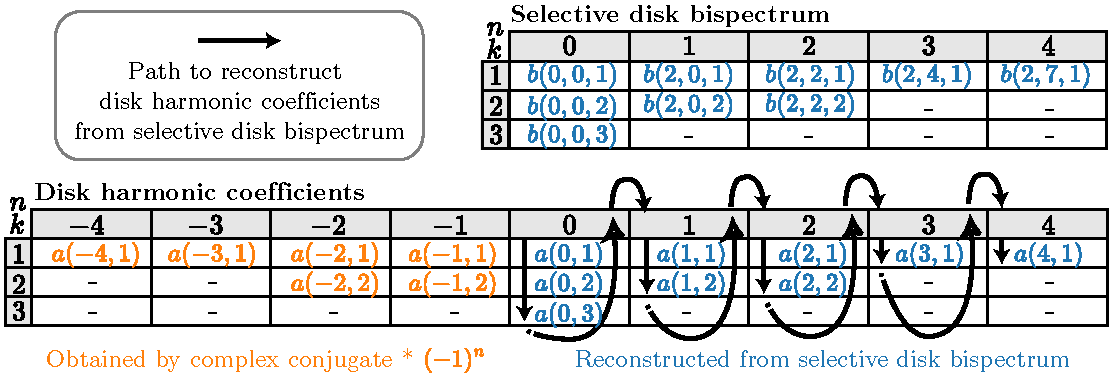
\includegraphics[width=0.9\linewidth]{figs/inversion.pdf}
  \caption{Graphical illustration of the selective disk bispectrum inversion. The arrows indicate in which order the DH coefficients are reconstructed.}
  \label{fig:bispecrum_inversion}
\end{figure}

We note that our inversion of the selective disk bispectrum also yields an inversion method for the (full) disk bispectrum. We also note that nonzero coefficient assumptions (such as $a_{n, 1} \neq 0$) are classic in bispectrum inversion literature to avoid division by zero. However, this assumption does not impact real-world application as long as there is some noise on the images.

\begin{theorem}[Complete Invariance]
Let \( f \) and \( f' \) be a pair of real-valued, square-integrable functions on the disk. Let the bispectrum be defined as in Definition~\ref{def:selective-bsp}. Assume that the DH coefficients \( a_{n,1} \) of \( f \) are non-zero for all \( n \in \{0, \dots, N_m - 1\} \). Then $b^f = b^{f'}$ if and only if \( f' = f \circ R_\phi \) for any 2D rotation \( \phi \in SO(2) \). Thus, the selective bispectrum is a complete invariant.
\end{theorem}

Part of the proof relies on the equivariance of the DH coefficients, which allow us to (re)prove the invariance of the (selective) disk bispectral coefficients used in~\citep{zhao2014rotationally}. The completeness of the SDB is proven by our inversion theorem, as the SDB contains all information about the original signal necessary for reconstruction.

\begin{figure*}[t]
  \centering
  \includegraphics[width=\textwidth]{figs/bispectrum_tractability.pdf}
  \caption{(a) The selective disk bispectrum (SDB) map is significantly faster than the full disk bispectrum map, especially for large images. (b) Bispectrum invariance error decreases with higher image resolution. (c-d) The SDB coefficient inversion sucessfully reconstructs images for resolution $28\times28$ (c) and $112\times112$ (d), and achieves a similar reconstruction error as the DH Transform \cite{fast_dhcs_2023} inversion.}
  \label{fig:tractability}
\end{figure*}


\subsection{Numerical Approximation of The Selective Disk Bispectrum and Its Inversion}

To further reduce the time complexity of the selective bispectrum, we propose leveraging a recent numerical approximation of the DH coefficients \citep{fast_dhcs_2023} which computes the disk harmonic transform in $O(L^2 \log L)$. This yields the following result:

\begin{proposition}[Complexity of the selective disk bispectrum]
    Denote $L \times L$ the size of the image, $m$ the number of DH coefficients. The time complexity of the approximate selective disk bispectrum is $O(L^2 \log L + m)$.
\end{proposition}

Next, we prove that we still have precise guarantees on the accuracy of the bispectrum coefficient approximations, the invariance property, and the reconstruction of the original image.

\begin{theorem}\label{th:accuracy}
Let \( 0 < \varepsilon \leq 1 \) be a target accuracy, and assume that \( \lambda \leq \sqrt{\pi p} \) and \( |\log \varepsilon| \leq \sqrt{p} \), where $\lambda$ is the bandlimit for the DH coefficients and \( p = L^2 \) the number of pixels in the image $f$ of size $L \times L$. Let \( b^f \) and \( \tilde{b}^f \) denote the exact and approximate selective disk bispectrum of \( f \), where \( \tilde{b}^f \) is computed using the approximate disk harmonic transform of \citet{fast_dhcs_2023}. Then,
\[
\| \tilde{b}^f - b^f \|_{\infty} \leq C\varepsilon \| f \|_{1},
\]
for a constant \( C \) depending only on a bound of \( f \) on its compact disk support.
\end{theorem}

As a corollary, we find that the bispectrum coefficients are approximately invariant with controlled guarantees.

\begin{corollary}
    Let $f, f'$ be a pair of real-valued square integrable functions on the disk such that there exists a $\phi \in SO(2)$ such that $f' = f \circ R_\phi$. Under the notations and assumptions of Theorem~\ref{th:accuracy}, we have:
    \begin{equation}
        \| \tilde b^{f} - \tilde b^{f'}\|_\infty \leq 2C \varepsilon \|f\|_1,
    \end{equation}
    for a constant \( C \) depending only on a bound of \( f \) on its compact disk support.
\end{corollary}

Linking the accuracy to $f$ is useful, as it allows us to control accuracy through number of pixels $p$. If $|f|$ and $C$ are large, but we still want to reach a given accuracy, then we can choose $p$ accordingly such that $\log(\epsilon) < \sqrt{p}$) to match the desired accuracy.

\subsection{MRA with the Selective Disk Bispectrum}

We follow \cite{bendory2018bispectrum}'s assumption that $\mathbb{E}[b_i] = b^f + \delta$, where $b_i \in \{b_1, ..., B_I\}$ is the bispectrum of one rotated noisy observation, $b^f$ is the bispectrum of the true signal $f$, and $\delta$ is a bias term introduced by noise propagation in bispectrum space. In this setting, we derive $\delta$ in the setting where $b^f$ is the disk bispectrum.

\begin{proposition}[SDB MRA Correction]
     When performing MRA using the selective disk bispectrum of noisy rotated images, the mean bispectrum must be corrected by subtracting $\delta$ before inversion to image space.
     \begin{equation}
         \delta = \sigma^2[S^\dagger_{0, k_3}  \delta_{n_{j_1},0}\delta_{n_{j_2},0} + S_{01}     \delta_{1, k_3}\delta_{n_{j_2},0}+ S_{01} \delta_{1, k_3}\delta_{n_{j_1},0}]
     \end{equation}
     \label{eq:mra-correction}

\end{proposition}

\section{Tractability of Selective Disk Bispectrum}
\label{sec:tractability}

\begin{figure*}[t]
  \centering
   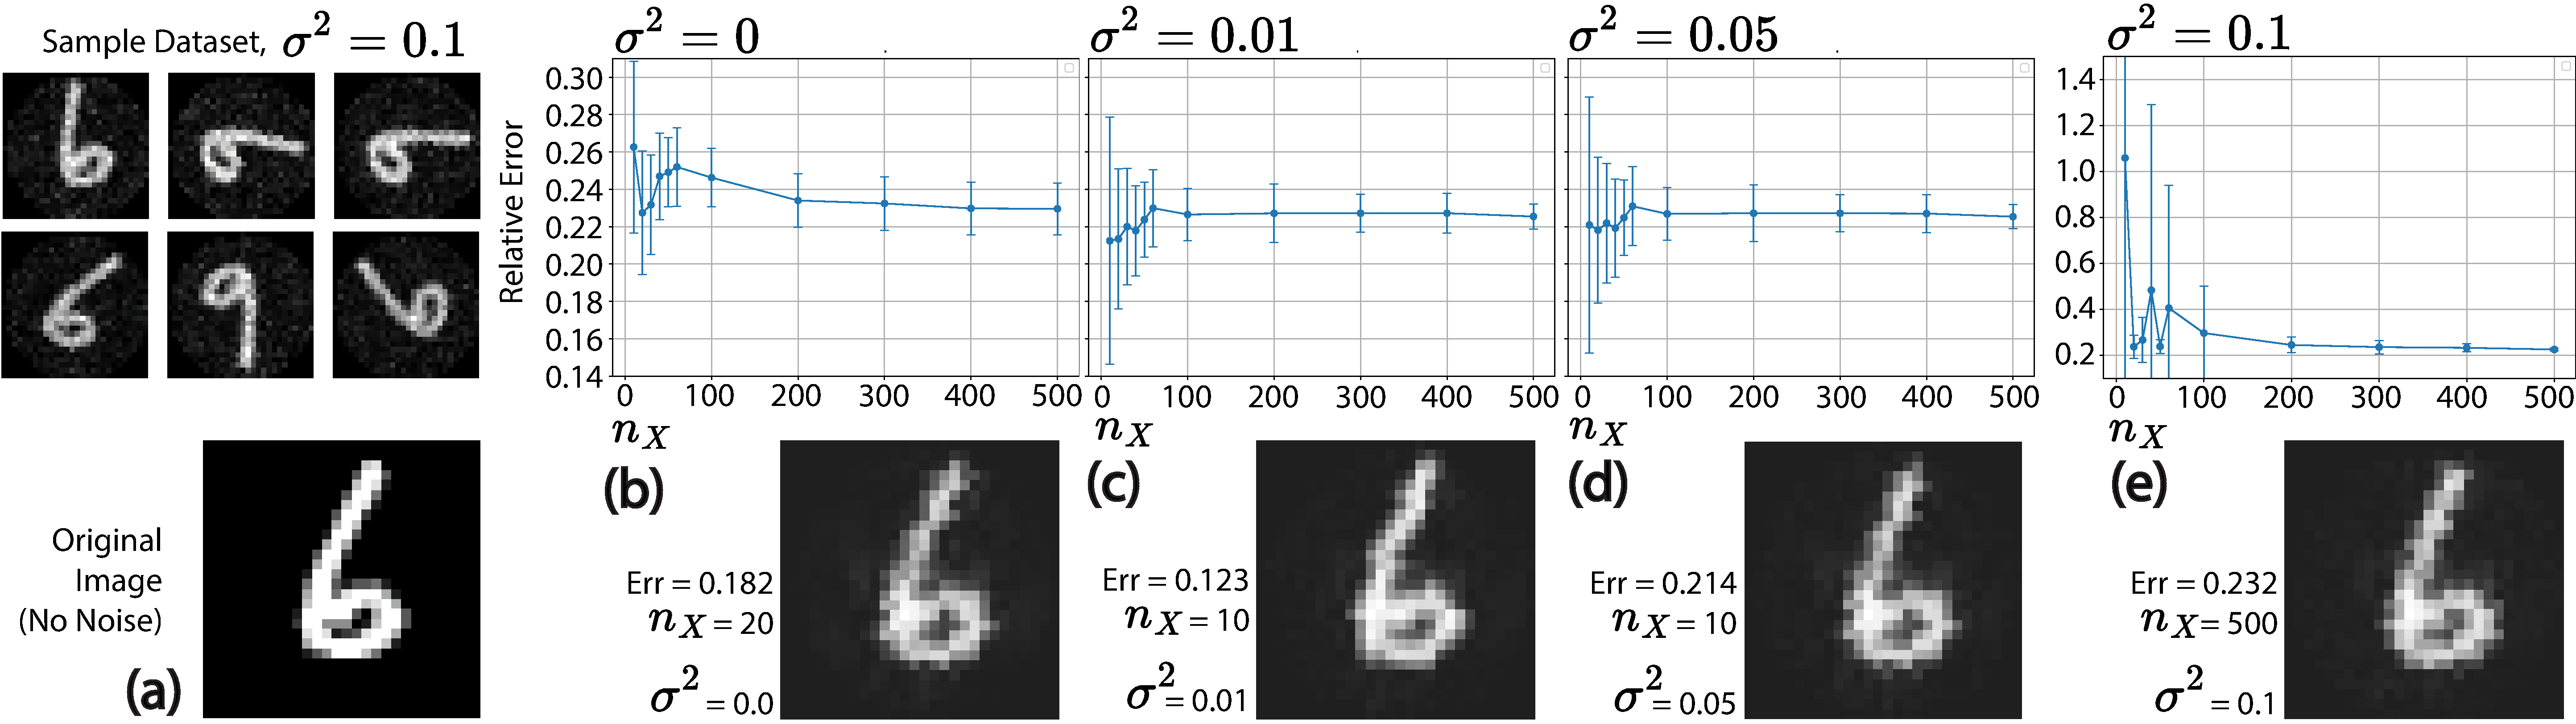
\includegraphics[width=\textwidth]{figs/mra_results.pdf}
    \caption[width=\textwidth]{(a) Dataset samples and original image used in MRA experiments for MNIST 6. (b-e) Relative error compares the similarity between the MRA reconstructed image and the original image used to generate the noisy rotated dataset for (b) $\sigma^2 = 0$ (c) $\sigma^2 = 0.01$, (d) $\sigma^2 = 0.05$, (e) $\sigma^2 = 0.1$. Sample reconstructions are shown below each result plot.}
    \label{fig:widecaption}

   \label{fig:mra-results}
\end{figure*}

To illustrate the computational and representational properties of our proposed selective disk bispectrum, we conduct a series of experiments testing \textit{speed}, \textit{invertibility}, and \textit{rotation invariance}. We compare against the full disk bispectrum proposed by \citep{zhao2014rotationally} and described in Eq. \ref{eq:disk_bispectrum}. Both the full and selective bispectra are computed using the disk harmonic coefficient library implemented by \citep{fast_dhcs_2023} on a MacBook Pro with an Apple M2 Max chip.

\subsection{Design of Tractability Experiments}

We consider square grayscale palm tree images of length \( L \in \{16 , 28, 56, 112\} \), each perturbed with Gaussian noise of standard deviation \( \sigma \in \{0, 0.01, 0.05, 0.1\} \). For each image, we compute both the full and selective disk bispectrum using the formulations in Eq.~\ref{eq:disk_bispectrum} (full) and Eq.~\ref{eq:selective_disk_bispectrum} (selective). We repeat these experiments for all digits of MNIST, and show results in the Appendix.

\textbf{Speed.} We compare the runtime of the forward and inverse bispectrum transforms across image sizes $L$ and noise levels $\sigma$. The full disk bispectrum is computationally expensive and impractical for many cases. In contrast, our \emph{selective disk bispectrum} enables efficient computation, making both encoding and reconstruction feasible even for larger images.

\textbf{Invertibility.} In the previous section, we prove that the selective disk bispectrum is \textit{complete}. Here, we visually confirm our theoretical results by constructing an image \( f \) from its bispectrum and measuring the relative reconstruction error $\varepsilon_{\text{rel}} = \frac{\left\lVert \hat{f} - f \right\rVert}{\left\lVert f \right\rVert}$, where \( \hat{f} \) is the image reconstruction obtained by applying the inverse map to the disk bispectrum coefficients. We observe in Fig. \ref{fig:tractability} that the selective bispectrum retains the essential information needed to accurately reconstruct the original image, demonstrating its practical completeness.

% \[
% \varepsilon_{\text{rel}} = \frac{\left\lVert \hat{f} - f \right\rVert}{\left\lVert f \right\rVert},
% \]

\textbf{Rotation Invariance.} We verify the invariance of the disk bispectrum to disk rotations. Given an image \( f \) and its rotated version \( f' \), we compute their respective bispectra \( b^{f} \) and \( b^{f'} \). Since the bispectrum is designed to be invariant to rotations, we expect $b^{f} = b^{f'}$. To quantify invariance, we compute the relative error between the two bispectra $\varepsilon_{\text{rel}} = \frac{\left\lVert b^{f} - b^{f'} \right\rVert}{\left\lVert b^{f} \right\rVert}$. Low error values across test conditions confirm that both the full and selective bispectra exhibit strong empirical rotation invariance, as shown in Fig.~\ref{fig:tractability}.
% \[
% \varepsilon_{\text{rel}} = \frac{\left\lVert b^{f} - b^{f'} \right\rVert}{\left\lVert b^{f} \right\rVert}.
% \]

\subsection{Results of Tractability Experiments}

We present the results of the tractability experiments. Full experimental results, including results on all MNIST images, are available in the Appendix.

\textbf{Speed.} The selective disk bispectrum offers a 3× speedup over the full bispectrum for \(16 \times 16\) images, and a 17,\!322× speedup for \(112 \times 112\) images. The inverse transform is equivalently fast for the full and selective bispectra, since the full bispectrum inversion utilizes only the subset of its coefficients included in the selective variant. Forward and inverse timing results are shown in Fig.~\ref{fig:tractability} for \(\sigma = 0\); run times are unaffected by noise level.

\textbf{Invariance.} Bispectrum invariance error decreases with higher image resolution, as shown in Fig.~\ref{fig:tractability}, and is as low as $3$ percent for $112\times112$ images. Invariance error is largely unaffected by noise level.

\textbf{Invertibility.} As shown in Fig.~\ref{fig:tractability}, the selective bispectrum accurately reconstructs the original image. This reconstruction accuracy is identical to the full bispectrum's. While reconstruction error increases slightly at lower tested resolutions, images are sufficiently reconstructed across all tested settings (see Appendix for reconstruction across bispectrum type, noise, and image resolution). Importantly, bispectrum inversions match the original image, up to a rotation. Since the bispectrum inversion reconstructs the original image up to a global rotation, reconstructions in Fig. ~\ref{fig:tractability} have been manually registered to match the orientation of the original image for clear comparison.

\section{Application: Multi-Reference Alignment with the Selective Disk Bispectrum}

We demonstrate the utility of our S. D.B. and its inversion for rotation-invariant multi-reference alignment (MRA), leveraging our new MRA correction term. We test rotation-invariant MRA on all MNIST digits, with results for the digit \textit{6} shown in Fig.~\ref{fig:mra-results} and other digits in the Appendix. For each experiment, we begin with a noiseless MNIST image and generate
\( n_X \in \{10, 20, 30, 40, 50, 60, 100, 200, 300, 400, 500\} \) copies. Each copy is corrupted with i.i.d.\ Gaussian noise
\( n \sim \mathcal{N}(0, \sigma^2) \) for
\( \sigma^2 \in \{0, 0.01, 0.05, 0.1\} \), randomly rotated by
\( R \in [0, 2\pi] \), and masked outside the disk, yielding
\( n_X \) images \( \{\tilde{f}_i\}_{i=1}^{n_X} \). We map each image to bispectrum space to obtain \( \{b_i\}_{i=1}^{n_X} \), average the bispectra, apply our correction term from Eq.~\ref{eq:mra-correction}, and map the corrected average back to image space using our disk bispectrum inversion method from Sec.~\ref{sec:theory}. Each experiment is repeated ten times with different random seeds, and computes relative error between MRA estimate $\bar{f}$ and true signal $f$ as $\varepsilon_{\text{rel}} = \frac{\left\lVert \bar{f} - f \right\rVert^2}{\left\lVert f \right\rVert^2}$. As shown in Fig.~\ref{fig:mra-results}, reconstruction error decreases and stabilizes around 0.23 as \( n_X \) increases—consistent with the empirical baseline reconstruction and invariance errors reported for $28\times28$ images in Sec.~\ref{sec:tractability}. These results are the first demonstration of MRA using a rotation-invariant bispectrum.

\section*{Conclusion}

We present the first disk bispectrum inversion, which reveals the minimal sufficient coefficients needed for accurate shape recovery. This enables the construction of our \emph{selective} disk bispectrum, which is \textbf{17,322× faster} to compute than the full bispectrum for $(122\times112)$ images. Crucially, our disk bispectrum inversion provides a mapping from disk bispectrum coefficients back to the image they represent, meaning that statistics can be done in bispectrum space and the result can be mapped back to image space. Without this, methods such as MRA would be impossible. Accordingly, we additionally derive the noise propagation that would occur for selective disk bispectrum MRA (in line with \cite{bendory2018bispectrum} and use it to showcase our bispectrum inverse in MRA experiments. The selective disk bispectrum's speed and invertibility position it as a tractable and scalable shape representation for rotation-invariant learning.

{
    \small
    \bibliographystyle{ieeenat_fullname}
    \bibliography{main}
}

% WARNING: do not forget to delete the supplementary pages from your submission
% \input{sec/X_suppl}

\end{document}
